
\section{QUY TẮC ĐẾM}

\subsubsection{Quy tắc cộng và sơ đồ hình cây}
\begin{itemize}
	\item [\iconMT] \indam{ Quy tắc cộng:} 
	\begin{tcolorbox}[colframe=orange,colback=orange!3,boxrule=0.2mm]
		Giả sử một công việc được hoàn thành bởi một trong \textbf{hai} phương án khác nhau: 
		\begin{itemize}
			\item [$\bullet$] Phương án 1 có $n_1$ cách thực hiện; 
			\item [$\bullet$] Phương án 2 có $n_2$ cách thực hiện không trùng hành động thứ nhất.
		\end{itemize}
		Khi đó, số cách thực hiện công việc là $n_1+n_2$ cách.
	\end{tcolorbox}
	\item [\iconMT] \indam{Sơ đồ hình cây:}
		\immini{
				Là sơ đồ bắt đầu tại một nút duy nhất với các nhánh tỏa ra các nút bổ sung.
				Trong các bài toán đếm, ta thường dùng sơ đồ hình cây để minh họa, giúp cho việc đếm thuận tiện và không bỏ sót trường hợp.
	 }
		{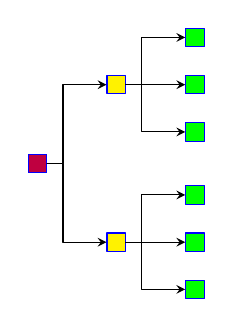
\begin{tikzpicture}[font=\footnotesize, line join=round, line cap=round, >=stealth,scale=2]
				\path(0,0)node(a)[draw=blue,fill=purple]{}
				++(0.5,0.5)node[draw=blue,fill=yellow](b){}
				(a)++(0.5,-0.5)node[draw=blue,fill=yellow](c){}
				;
				\path
				(b)++(0.5,0.3)node(b1)[draw=blue,fill=green]{ }
				(b)++(0.5,0)node(b2)[draw=blue,fill=green]{ }
				(b)++(0.5,-0.3)node(b3)[draw=blue,fill=green]{}
				;
				\path
				(c)++(0.5,0.3)node(c1)[draw=blue,fill=green]{ }
				(c)++(0.5,0)node(c2)[draw=blue,fill=green]{ } 
				(c)++(0.5,-0.3)node(c3)[draw=blue,fill=green]{ }
				;
				\draw[-stealth,outer sep=0,inner sep=0](a.east)--++(0.1,0)|-(b.west);
				\draw[-stealth,outer sep=0,inner sep=0](a.east)--++(0.1,0)|-(c.west);
				\draw[-stealth,outer sep=0,inner sep=0](b.east)--++(0.1,0)|-(b1.west);
				\draw[-stealth,outer sep=0,inner sep=0](b.east)--++(0.1,0)|-(b2.west);
				\draw[-stealth,outer sep=0,inner sep=0](b.east)--++(0.1,0)|-(b3.west);
				\draw[-stealth,outer sep=0,inner sep=0](c.east)--++(0.1,0)|-(c1.west);
				\draw[-stealth,outer sep=0,inner sep=0](c.east)--++(0.1,0)|-(c2.west);
				\draw[-stealth,outer sep=0,inner sep=0](c.east)--++(0.1,0)|-(c3.west);
		\end{tikzpicture}}
\end{itemize}

\subsubsection{Quy tắc nhân}
\begin{itemize}
	\item [\iconMT] \indam{Quy tắc nhân:} 
	\begin{tcolorbox}[colframe=orange,colback=orange!3,boxrule=0.2mm]
		Giải sử một công việc được hoàn thành bởi \textbf{hai} công đoạn \textbf{liên tiếp} nhau:
		\begin{itemize}
			\item [$\bullet$] Công đoạn 1 có $m_1$ cách thực hiện, 
			\item [$\bullet$] Với mỗi cách thực hiện công đoạn 1, có  $m_2$ cách thực hiện công đoạn 2.
		\end{itemize}
		Khi đó, số cách thực hiện công việc là $m_1 \cdot m_2$ cách.
	\end{tcolorbox}
	\item [\iconMT] \indam{Lưu ý:} Quy tắc nhân áp dụng để tính số cách thực hiên công việc có nhiều công đoạn, các công đoạn nối tiếp nhau và những công đoạn này độc lập nhau.
\end{itemize}
